\usetikzlibrary{arrows}
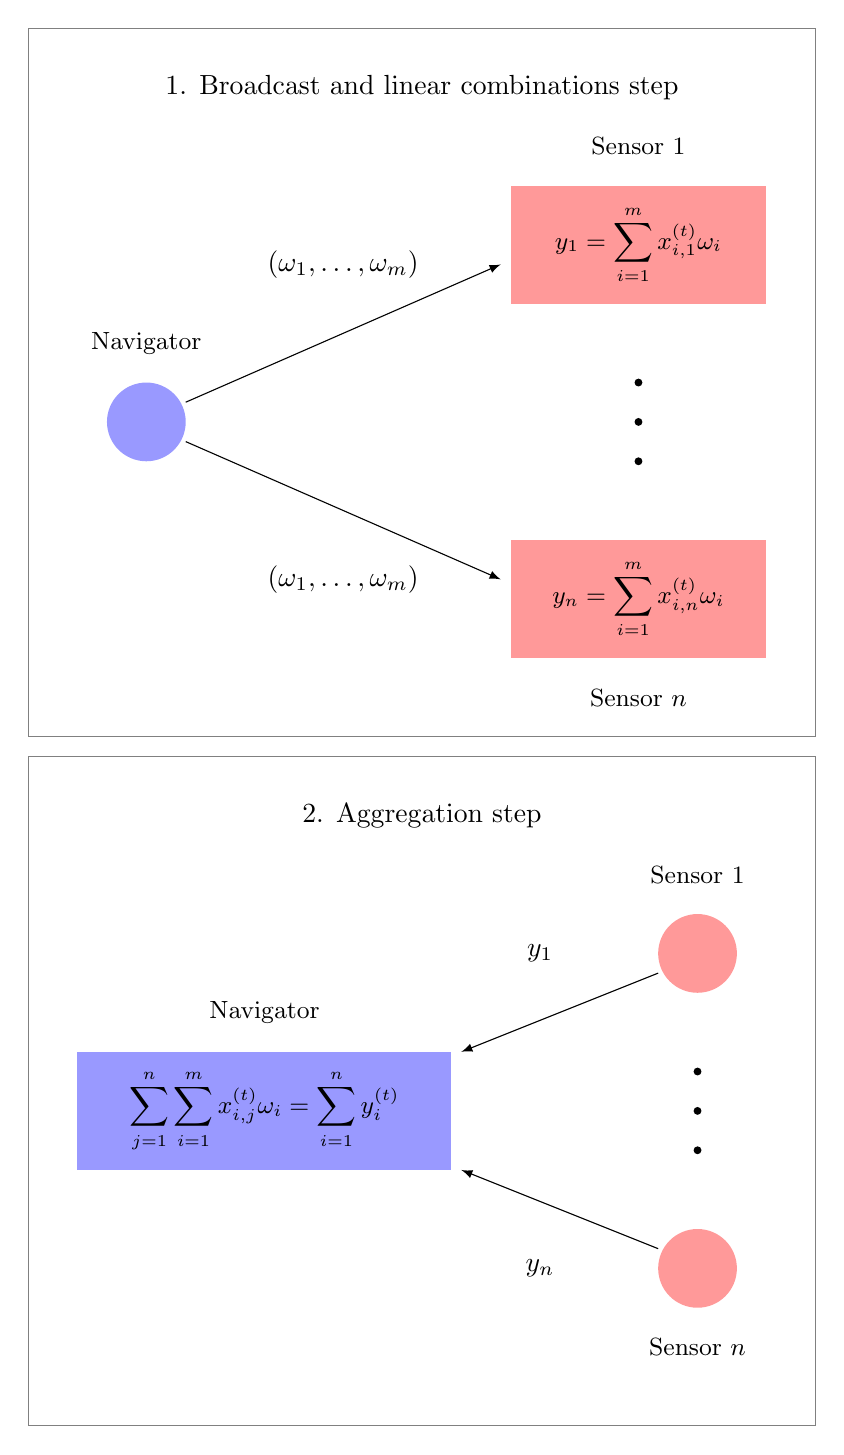
\begin{tikzpicture}
    % Step 1
    \node at (5,22.5) {1. Broadcast and linear combinations step};
    % Navigator
    \node at (1.5,19.25) {\small Navigator};
    \fill (1.5,18.25) [fill=blue!40] ellipse (0.5 and 0.5);
    % Sensors
    \node at (7.75,21.75) {\small Sensor $1$};
    \fill [fill=red!40] (6.125,19.75) rectangle (9.375,21.25);
    \node at (7.75,20.5) {\small $\displaystyle y_1 = \sum^m_{i=1}x_{i,1}^{(t)}\omega_i$};
    \node at (7.75,14.75) {\small Sensor $n$};
    \fill [fill=red!40] (6.125,15.25) rectangle (9.375,16.75);
    \node at (7.75,16) {\small $\displaystyle y_n = \sum^m_{i=1}x_{i,n}^{(t)}\omega_i$};
    \fill [black] (7.75,18.75) circle (0.05);
    \fill [black] (7.75,17.75) circle (0.05);
    \fill [black] (7.75,18.25) circle (0.05);
    % Lines
    \draw [-latex] plot[smooth, tension=.7] coordinates {(2,18.5) (6,20.25)};
    \draw [-latex] plot[smooth, tension=.7] coordinates {(2,18) (6,16.25)};
    \node at (4,20.25) {$(\omega_1,\dots ,\omega_m)$};
    \node at (4,16.25) {$(\omega_1,\dots ,\omega_m)$};
    
    % Step 2
    \node at (5,13.25) {2. Aggregation step};
    % Navigator
    \node at (3,10.75) {\small Navigator};
    \fill [fill=blue!40] (0.625,8.75) rectangle (5.375,10.25);
    \node at (3,9.5) {\small $\displaystyle \sum^{n}_{j=1}\sum^{m}_{i=1} x_{i,j}^{(t)}\omega_i = \sum^n_{i=1}y^{(t)}_{i}$};
    % Sensors
    \node at (8.5,12.5) {\small Sensor $1$};
    \fill  (8.5,7.5) [fill=red!40] ellipse (0.5 and 0.5);
    \node at (8.5,6.5) {\small Sensor $n$};
    \fill  (8.5,11.5) [fill=red!40] ellipse (0.5 and 0.5);
    \fill [black] (8.5,10) circle (0.05);
    \fill [black] (8.5,9) circle (0.05);
    \fill [black] (8.5,9.5) circle (0.05);
    % Lines
    \draw [-latex] plot[smooth, tension=.7] coordinates {(8,11.25) (5.5,10.25)};
    \draw [-latex] plot[smooth, tension=.7] coordinates {(8,7.75) (5.5,8.75)};
    \node at (6.5,11.5) {$y_1$};
    \node at (6.5,7.5) {$y_n$};
    
    % Bounding rectangles
    \draw [gray] (0,23.25) rectangle (10,14.25);
    \draw [gray] (0,14) rectangle (10,5.5);
\end{tikzpicture}